\documentclass[10pt,a4paper]{article} % Reduce font size for compactness
\usepackage[utf8]{inputenc}
\usepackage{geometry}
\geometry{a4paper, margin=0.75in} % Adjust margins for print optimization
\usepackage{enumitem}
\usepackage{hyperref}
\usepackage{graphicx} % Required for including a photo
\usepackage{multicol} % Optional: Two-column layout
\usepackage{parskip} % Remove paragraph indentation
\setlength{\parskip}{0.2em} % Fine-tune paragraph spacing
\setlength{\itemsep}{0pt} % Reduce item spacing in lists

\begin{document}

% Personal Information
\begin{center}
    \begin{minipage}{0.7\textwidth}
        \textbf{\Large Ran Tian} \\
        \href{mailto:tianran.haru@gmail.com}{tianran.haru@gmail.com}\\
        \href +44 07436644896 \\
        \href{www.linkedin.com/in/rantianharu}{www.linkedin.com/in/rantianharu}\\
        \href{https://github.com/HaruTian4604}{https://github.com/HaruTian4604}
    \end{minipage}
    \hfill
    \begin{minipage}{0.25\textwidth}
        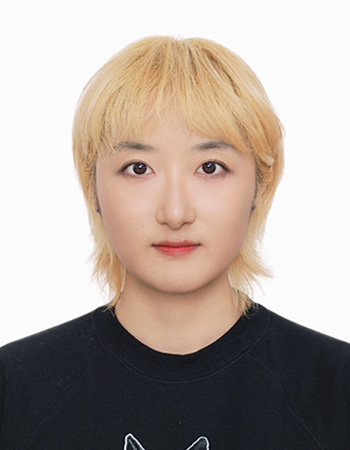
\includegraphics[width=1.0\linewidth]{RanTianPhoto.JPEG} % Add your photo file here
    \end{minipage}
\end{center}

% Personal Profile
\section*{Personal Profile}
Computer Science MSc student with a background in hospitality management, bringing a unique perspective to software development. Passionate about writing clean, maintainable code and designing intuitive software solutions. Proficient in C, Java, and experienced in applying software engineering best practices, including version control, agile development, and test-driven development. Hands-on experience in building applications that balance functionality and aesthetics. Developed strong problem-solving skills through technical projects and honed leadership and communication abilities as a class representative. Seeking an entry-level software development role where I can combine technical expertise with user-centric design to create efficient, elegant, and scalable solutions.

% Education
\section*{Education}

\textbf{University of Bristol, MSc Computer Science (Conversion)} \hfill \textbf{Sep 2024 - Sep 2025} \\
Relevant coursework: C Programming, Software Engineering, Java OOP, Git, SQL, Web Tech, Computer Architecture

\textbf{Edinburgh Napier University (Singapore Campus), BSc (Hons) Hospitality and Tourism Management} \hfill \textbf{Jul 2019 - Nov 2022} \\

\textbf{SHATEC (Singapore Hotel and Tourism Education Centre), Diploma in Hotel Management} \hfill \textbf{Apr 2015 - Dec 2017} \\

% Skills
\section*{Skills}

\textbf{Technical:} Backend/frontend development, Git, UI/UX, responsive design, web technologies. \\
\textbf{Languages:} C, Java, JavaScript, HTML, CSS, SQL, P5.js \\
\textbf{Soft Skills:} Teamwork, problem-solving, adaptability, leadership, time management.

% Projects
\section*{Projects}

\subsection*{Database Management System (Java, SQL)}
\begin{itemize}
    \item Designed a \textbf{DBMS} with SQL-like query execution and indexing for efficient data retrieval.
    \item Implemented \textbf{persistent storage} and \textbf{error handling} to ensure data integrity.
    \item Applied \textbf{OOP} and \textbf{TDD} for maintainability and robustness.
\end{itemize}

\subsection*{Dino Escape Game (p5.js, Agile)}
\begin{itemize}
    \item Developed a \textbf{browser-based survival game} using p5.js with real-time interactions.
    \item Followed \textbf{Agile methodologies} and used Git for version control.
    \item Implemented \textbf{game mechanics} such as health depletion and resource collection.
    \item Project Link: \href{https://github.com/UoB-COMSM0166/2025-group-13}{https://github.com/UoB-COMSM0166/2025-group-13}
\end{itemize}

\subsection*{Emergency Migration Management System (Java, SQL, UI/UX) | Personal Project (Planned Summer 2025)}
\begin{itemize}
    \item Researched inefficiencies in real-world government systems (e.g., UK's "Homes for Ukraine").
    \item Designed a \textbf{database-driven system} for refugee placement and data management.
    \item Created \textbf{data visualization prototypes} to enhance usability and reporting.
\end{itemize}

% Work Experience
\section*{Work Experience}

\textbf{Course Representative} \hfill \textbf{University of Bristol, Sep 2024 - Present} \\
\begin{itemize}
    \item Served as the primary liaison between students and faculty, advocating for academic improvements.
    \item Collected and presented student feedback and collaborated with faculty on curriculum enhancements.
\end{itemize}

\textbf{Marketing Planner \& Frontend Developer} \hfill \textbf{Shanghai Electric Technology (China), Aug 2021 - May 2023} \\
\begin{itemize}
    \item Led website development and social media campaigns, increasing brand visibility.
\end{itemize}

\textbf{Software Prototyping \& Digital Marketing Specialist \& Frontend Developer} \hfill \textbf{Nsecsoft (China), Mar 2019 - Aug 2021} \\
\begin{itemize}
    \item Developed and maintained company websites, improving UX and accessibility.
    \item Designed UI prototypes using Axure and optimized front-end performance.
    \item Project Link: \href{https://www.nsecsoft.com/}{https://www.nsecsoft.com/}
\end{itemize}

\end{document}
